\documentclass{article}

% if you need to pass options to natbib, use, e.g.:
\PassOptionsToPackage{numbers, compress}{natbib}
% before loading nips_2016
%
% to avoid loading the natbib package, add option nonatbib:
% \usepackage[nonatbib]{nips_2016}

%\usepackage{nips_2016}

% to compile a camera-ready version, add the [final] option, e.g.:
\usepackage[final]{nips_2016}

\usepackage[utf8]{inputenc} % allow utf-8 input
\usepackage[T1]{fontenc}    % use 8-bit T1 fonts
\usepackage{hyperref}       % hyperlinks
\usepackage{url}            % simple URL typesetting
\usepackage{booktabs}       % professional-quality tables
\usepackage{amsfonts}       % blackboard math symbols
\usepackage{nicefrac}       % compact symbols for 1/2, etc.
\usepackage{microtype}      % microtypography
\usepackage{amsmath}        % equations
\usepackage{color}
\usepackage{graphicx}
\usepackage{subcaption}


\title{Temporal Activity Detection in Untrimmed Videos with Recurrent Neural Networks}

% The \author macro works with any number of authors. There are two
% commands used to separate the names and addresses of multiple
% authors: \And and \AND.
%
% Using \And between authors leaves it to LaTeX to determine where to
% break the lines. Using \AND forces a line break at that point. So,
% if LaTeX puts 3 of 4 authors names on the first line, and the last
% on the second line, try using \AND instead of \And before the third
% author name.

\author{
    Alberto Montes \\
    Universitat Politècnica de Catalunya \\
    Barcelona, Spain \\
    \texttt{al.montes.gomez@gmail.com} \\
    \And
    Amaia Salvador \\
    Image Processing Group \\
    Universitat Politècnica de Catalunya \\
    Barcelona, Spain \\
    \texttt{amaia.salvador@upc.edu} \\
    \And
    Xavier Giro-i-Nieto \\
    Image Processing Group \\
    Universitat Politècnica de Catalunya \\
    Barcelona, Spain \\
    \texttt{xavier.giro@upc.edu} \\
}

\begin{document}
% \nipsfinalcopy is no longer used

\maketitle

\begin{abstract}

% AMAIA: La primera frase de l'abstract potser no cal, ja que és massa introductoria. L'he comentat i modificat l'abstract

    This work proposes a simple pipeline to classify and temporally localize activities in untrimmed videos. Our system uses features from a 3D Convolutional Neural Network (3D-CNN) as input to train a a recurrent neural network (RNN) that learns to classify video clips of 16 frames. After clip prediction, we post-process the output of the RNN to assign a single activity label to each video, and determine the temporal boundaries of the activity within the video. We show how our system can achieve competitive results in both tasks with a simple architecture. We evaluate our method in the ActivityNet Challenge 2016, achieving a 0.5874 mAP and a 0.2237 mAP in the classification and detection tasks, respectively. Our code and models are publicly available at at: \url{https://github.com/imatge-upc/activitynet-2016-cvprw}

%AMAIA: s'han d'afegir els valors de mAP (o la metrica que sigui).
%ALBERTO: FET
\end{abstract}

\section{Introduction}

Recognizing activities in videos has become a hot topic over the last years due to the continuous increase of video capturing devices and online repositories.
This large amount of data requires an automatic indexing to be accessed after capture.
The recent advances in video coding, storage and computational resources have boosted research in the field towards new and more efficient solutions for organizing and retrieving video content.

Impressive progress has been reported in the recent literature for video classification~\cite{tran2014learning,tran2015deep,wang2015towards,yao2015describing}, which requires to assign a label for the input video. While this task is already challenging, it typically requires videos to be trimmed beforehand (i.e. the category is present in the entire video).
However, a video classification system should be able to recognize activities in untrimmed videos, and find the temporal segments in which they appear.
This second challenge has been recently proposed in the ActivityNet Challenge 2016~\cite{caba2015activitynet}, in which participants are asked to both provide a single activity for each video, as well as the temporal segment where the activity happened in the video.
% AMAIA: Amb això et refereixes que la tasca de detecció temporal es nova d'Activitynet? Ho he modificat una mica... No queda massa clar... Si és així, jo directament mencionaria la challenge i la citaria.
In order to face both these challenges at the same time, we propose a simple pipeline composed of a 3D-CNN that exploits spatial and short temporal correlations followed by a recurrent neural network which exploits long temporal correlations.

% AMAIA: Decidim si volem dir 'CNN' o 'ConvNet'. Ara ho he deixat tot amb CNN. Millor no barrejar

\section{Related work}

% AMAIA: El related work dels datasets me'l saltaria per guanyar espai. L'he comentat.

%The activity classification and temporal localization tasks have been proposed with datasets such as Sports1M~\cite{KarpathyCVPR14}, THUMOS~\cite{THUMOS15} or ActivityNet~\cite{caba2015activitynet} published in the recents years. Many frameworks have been proposed to solve this tasks.
Several works in the literature have used 2D-CNNs to exploit the spatial correlations between frames of a video by combining their outputs using different strategies~\cite{gkioxari2015contextual,yeung2015end,ballas2015delving}. Others have tried using the optical flow as an additional input to the 2D-CNN videos~\cite{wang2015towards}, which provides information of the temporal correlations. % AMAIA: Tot això s'ha de revisar...

Later on, 3D-CNNs were proposed in ~\cite{tran2014learning}, which were able to exploit short temporal correlations between frames and have demonstrated to work remarkably well for video classification~\cite{tran2014learning,tran2015deep}. 3D-CNNs have also been used for temporal detection in~\cite{shoutemporal}, where multi-stage 3D-CNN architecture is used to classify video segment proposals.

For temporal activity detection, recent works have proposed the usage of Long Short-Term Memory units (LSTM)~\cite{hochreiter1997long}.
LSTMs are a type of RNNs that is able to better exploit long and short temporal correlations in sequences, which makes them suitable for video applications.
LSTMs have been used alongside CNNs for video classification~\cite{yao2015describing} and activity localization in videos~\cite{yeung2015every}.

% AMAIA: Aquí falta una frase que digui què fem diferent nosaltres, en què ens assemblem a l'estat de l'art...

\section{Proposed Architecture}
% AMAIA: He tret això dels paràgrafs, ja que ocupen massa espai i no tenim tantes coses per explicar...

% AMAIA: Ja sé que són 4 pàgines...però crec que estaria bé posar la figura de l'arquitectura no?? Potser, per aprofitar l'espai, pots fer una figura doble (o triple), i en cada columna pots posar una cosa: e.g. 1. Arquitectura (figura 1.1 de la teva memoria) 2. exemples visuals(que mostrin un frame del video, prediccio i groundtruth). La figura que també m'agrada és la 4.10 o 4.11 de la memòria (potser no cal posar-la sencera), on expliques diferents prediccions (a vegades la detecció està bé pero la classe global no, o al revés...). Jo crec que aquestes figures t'ajudaran a explicar els resultats i conclusions. https://imatge.upc.edu/web/sites/default/files/pub/xMontes.pdf

% AMAIA: Pel tema de les figures, si veus que ocupa molt pots descartar-ne alguna... depen del que vulguis explicar a la secció d'experiments

We use the 3D-CNN model proposed in~\cite{tran2014learning} to extract features for all videos in the database. We split the videos in 16-frame clips and resize them to 171$\times$128 to fit the original model's desired input. Features from the second fully connected layer (fc6) are extracted for each video clip.

% AMAIA: Els detalls de la xarxa no calen, ja que no l'hem dissenyat nosaltres. Els comento

%This network conducts 3D convolutions/pooling which operates in spatial and temporal dimensions simultaneously, and therefore can capture both appearance and motion.
%All 3D pooling layers use a 2$\times$2 max pooling with stride 2 in spatial dimensions, the same kernel size as in the temporal dimension except the first pooling layer (\texttt{pool1}) which has kernel size 1 and stride 1. All 3D convolutional filters have kernel size 3 and stride 1 in all dimensions.
%The network architecture used is the same as in the original paper except that it has been decided to work on the next stage with the values obtained at the \texttt{fc6} layer as feature vector for each 16-frame clip. The specifications of the network layers as well as the number of kernels by layer is the following one: \texttt{conv1(64) - pool1 - conv2a(128) - pool2 - conv3a(256) - conv3b(256) - pool3 - conv4a(512) - conv4b(512) - pool4 - conv5a(512) - conv5b(512) - pool(5) - fc6(4096)}.

\subsection{Recurrent Neural Network}
\label{sec:architecture}
Next, we design a network that takes a sequence of 3D-CNN-f6 features from a video, and returns a sequence of class probabilities for each element in the sequence. We use LSTM layers, followed with dropout with $p = 0.5$ and a fully connected layer with a softmax activation. Figure~\ref{fig:global_pipeline} shows the proposed architecture. Different configurations of the number of LSTM layers and the number of cells have been tested and will be reviewed in the following sections.

\begin{figure}[ht]
\centering
\includegraphics[width=.5\linewidth]{img/schematic_pipeline}
\caption{Global architecture of the proposed pipeline.}
\label{fig:global_pipeline}
\end{figure}


%The recurrent network have the following architecture: \texttt{input(4096) - dropout(.5) - N $\times$ lstm(c) - dropout(.5) - softmax(K+1)}.

%\paragraph{Training.}
%To train the recurrent network with the extracted features, was found that most of the videos had a clip length larger than a valid timestep at training, so a stateful approach was used at training where the memory was not reset between batches and at the same batch position was placed the continuation of the features of the previous seen video.

% AMAIA: Això de stateful i tal no cal no?

\subsection{Post-Processing}
Given a video, the prediction of our model is sequence of class probabilities for each 16-frame video clip. From this output, we need to be able to predict the activity  and temporally localize it. We post-process the network's output to achieve that goal. First, to obtain the activity prediction for the whole video, we simply compute the mean over all video clips in the video. We then take the class with maximum predicted probability as the predicted class.

%\begin{equation}
%	p(x) = \frac{1}{T} \sum_i^{T} p_i(x)
%\end{equation}

%where $T$ is number of video clips of 16 frames in the video.
% AMAIA: No cal posar l'equació de la mitja...

To obtain the temporal localization of the predicted activity, we first apply a mean filter of $k$ samples to the predicted sequence to smooth the values through time (see equation~\ref{eq:smooth}). Then, the probability of activity (vs no activity) is computed for all samples of the sequence, being the activity probability the sum of all activity probabilities, and the no activity probability, the one assigned to the background class. Finally, a threshold $\gamma$ is set and all clips with probability higher than $\gamma$ are considered as part of the detected temporal segment for the previously assigned activity.

\begin{equation}
	\tilde{p}_i(x) = \frac{1}{2k} \sum_{j=i-k}^{i+k} p_i(x)
    \label{eq:smooth}
\end{equation}

% \begin{equation}
%     \label{eq:activity_probability}
% 	\tilde{p}^a_i = \sum_{x=1}^{N}\tilde{p}_i(x), \text{where } x = \begin{cases}
%         0, & \text{background class} \\
%         i, & 1 \leq i \leq N \text{ activity classes}
%     \end{cases}
% \end{equation}

% AMAIA: Aquesta equació està be ?? Vull dir, no cal posar where x = blabla..., és simplement la suma de les probabilitats de 1 a N no? De fet crec que tampoc cal posar-la... Ho he explicat al text. Potser podria quedar més clar...

\section{Experiments}

\subsection{Dataset}
For all our experiments we use the dataset provided in the ActivityNet Challenge 2016~\cite{caba2015activitynet}. This dataset contains 640 hours of video and 64 million frames. The ActivityNet dataset is composed of untrimmed videos, providing temporal annotations for the given ground truth class labels. The dataset is split in 50\% for training, 25\% for validation and 25\% for testing.

\subsection{Training}
We train the network described in Section~\ref{sec:architecture} with the negative log likelihood loss, assigning a lower weight to background samples to deal with dataset imbalance (see Equation~\ref{eq:loss}).

\begin{equation}
    L(p,q) = - \sum_x \alpha(x) p(x) \log (q(x)), \text{ where } \alpha(x) =
    \begin{cases}
        \rho, & x = \text{background instance}\\
        1,    & \text{otherwise}
    \end{cases}
    \label{eq:loss}
\end{equation}

where $q$ is the predicted probability distribution and $p$ the ground truth probability distribution. In our experiments, we set $\rho = 0.3$.

The network was trained with batches of 256 samples, back-propagating the error during 20 time-steps per sample.
The optimizer function used was the RMSprop~\cite{dauphin2015rmsprop} with a learning rate set to $10^{-5}$. In total the network was trained with 100 epochs.

% AMAIA: Aquí tambe hauries d'afegir el numero de iteracions (o epochs), learning rate, optimizer, batch size. Si el tens, el temps d'entrenament en la GPU que entrenessis.
% ALBERTO: FET


\subsection{Results}

The evaluation metric follows the one used in ActivityNet Challenge with regard to classification and temporal activity localization as a retrieval problem, evaluating the mAP.
For temporal localization, a prediction is marked correct only when it has the correct category and has IoU with ground truth instance larger than $0.5$.

\begin{table}[h]
    \parbox{.45\linewidth}{
        \centering
        \begin{tabular}{l|cc}
        \textbf{Architecture} & \textbf{mAP} & \textbf{Hit@3} \\
        \hline
        3 x 1024-LSTM & 0.5635 & 0.7437 \\
        2 x 512-LSTM & 0.5492 & 0.7364 \\
        1 x 512-LSTM & \bf0.5938 & \bf0.7576 \\
        \end{tabular}
        \vspace{.5cm}
        \caption{Results for classification task comparing different architectures.}
        \label{table:classification_by_architecture}
    }
    \hfill
    \parbox{.45\linewidth}{
        \centering
        \begin{tabular}{l|ccc}
        \textbf{$\gamma$} & \textbf{$k=0$} & \textbf{$k=5$} & \textbf{$k=10$} \\
        \hline
        0.2 & 0.20732 & \bf0.22513 & 0.22136 \\
        0.3 & 0.19854 & 0.22077 & 0.22100 \\
        0.5 & 0.19035 & 0.21937 & 0.21302 \\
        \end{tabular}
        \vspace{.2cm}
        \caption{mAP with an IOU threshold of $0.5$ comparing between values of $k$ and $\gamma$ on post-processing.}
        \label{table:detection_postprocessing_comparison}
    }
\end{table}

The first results are related with the network architecture. It has been tested with different number of layers and different number of cells having all the layers the same number of cells. The results can be found in Table~\ref{table:classification_by_architecture}.
This results indicate that all the networks presented high learning capacity over the data, but a little over-fitting was observed with the deeper architectures, obtainng the best results with a single layer of 512-LSTM cells.

Once the architecture has been chosen to obtain the best performance in the classification task, some experiments with different values of $k$ and $\gamma$ for the post-processing were performed.
At Table~\ref{table:detection_postprocessing_comparison} there are the results for the temporal activity localization task, where the effect of a mean smoothing filter can be seen, improving the localization.
%there is the results for the temporal activity localization task, where can be seen that the effect of a mean filter to smooth helps improving the localization.

In the Figure~\ref{fig:example_results} is shown some examples of the temporal localization prediction for some instances of the dataset. It can be seen how the predictions are continuous and smooth and mostly overlaps with the ground truth instances.

\begin{figure}[ht]
\centering
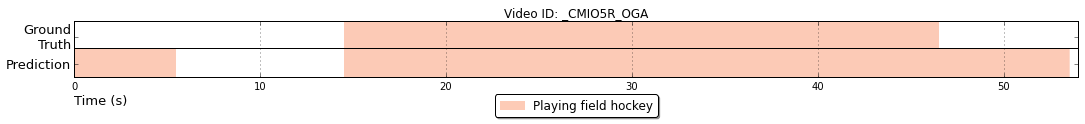
\includegraphics[width=1\linewidth]{img/activity_temporal_localization_8.png}
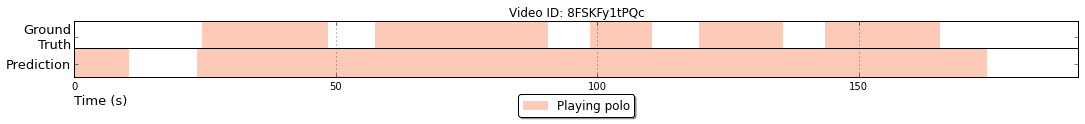
\includegraphics[width=1\linewidth]{img/activity_temporal_localization_11.png}
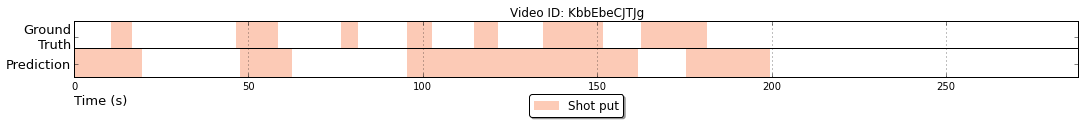
\includegraphics[width=1\linewidth]{img/activity_temporal_localization_20.png}
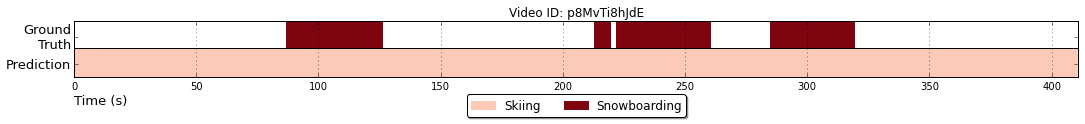
\includegraphics[width=1\linewidth]{img/activity_temporal_localization_35.png}

\caption{Global architecture of the proposed pipeline.}
\label{fig:example_results}
\end{figure}
% AMAIA: Crec que amb una secció on expliquis tots els experiments ja n'hi ha prou. Li he posat el nom de 'Results'

% AMAIA: Si aqui vols parlar del bias towards sport categories, hauries d'afegir la figura que tens que ho demostra.
% ALBERTO: crec que potser una segona figura no hi cab...posar-la a annexes potser???
\section{Conclusion}

We propose a simple pipeline which can be able to perform well in classification and temporal localization on activities on videos.
Moreover, the flexibility of this sequence to sequence prediction allows the proposed network to face tasks where more than a single activity is present in the video.

% ALBERTO: que més explico a les conclusions

In the future, we would like to extend the work training all the pipeline end-to-end, including the 3D-CNN and improve the accuracy obtained.

\section*{}
{\small
\bibliographystyle{plainnat}
\bibliography{references}
}

\end{document}
